\subsection{Computational Model}
\label{sec:resources}

This section pieces together a highly simplified model for a computer that
implements the Intel architecture, illustrated in
Figure~\ref{fig:computer_model}. The simplified model is intended to help the
reader's intuition process the concepts that the rest of the paper will build
on. The following sections gradually replace the simplified model with a more
accurate description of the Intel architecture.

\begin{figure}[hbt]
  \centering
  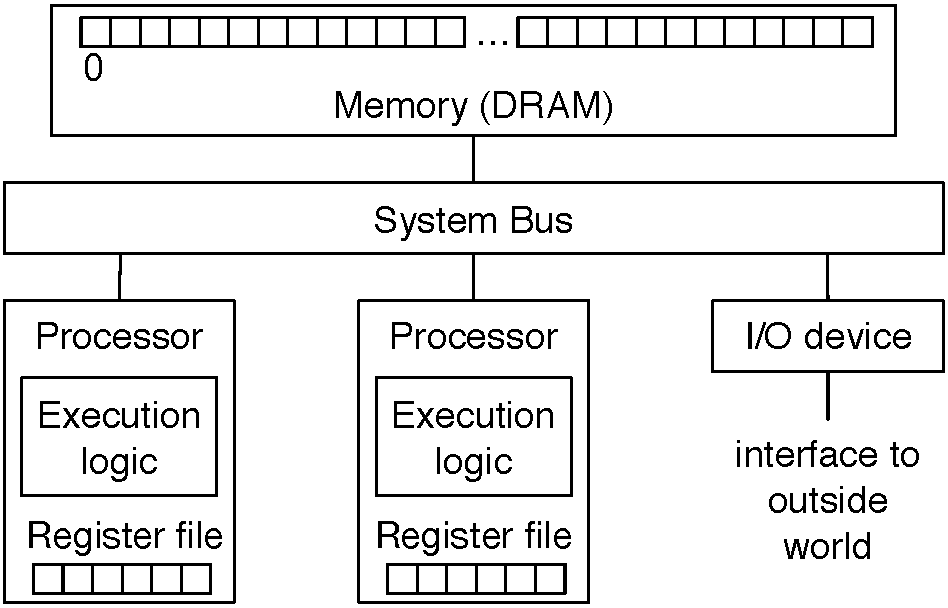
\includegraphics[width=65mm]{figures/computer_model.pdf}
  \caption{
    A computer's core is its processors and memory, which are connected by a
    system bus. Computers also have I/O devices, such as keyboards, which are
    also connected to the processor via the system bus.
  }
  \label{fig:computer_model}
\end{figure}


The building blocks for the model presented here come from
\cite{saltzer2009systemdesign}, which introduces the key abstractions in a
computer system then focuses on the techniques used to build software systems
on top of these abstractions

The memory is an array of storage cells, addressed using natural numbers
starting from 0, and implements the abstraction depicted in
Figure~\ref{fig:memory_abstraction}. Its salient feature is that the result of
reading the memory cell at an address must equal the most value written to that
memory cell.

\begin{figure}[hbt]
  \centering
  \begin{tabularx}{\columnwidth}{| X |}
  \hline
  \textsc{write}(\textit{addr}, \textit{value}) $ \rightarrow \varnothing $ \\
  Store \textit{value} in the storage cell identified by \textit{addr}. \\
  \hline
  \textsc{read}(\textit{addr}) $ \rightarrow $ \textit{value} \\
  Return the \textit{value} argument to the most recent \textsc{write} call
  referencing \textit{addr}. \\
  \hline
  \end{tabularx}
  \caption{The memory abstraction}
  \label{fig:memory_abstraction}
\end{figure}

A logical processor repeatedly fetches \textit{instructions} from the
computer's memory and executes them, according to the flowchart in
Figure~\ref{fig:processor_execution}.

\begin{figure}[hbt]
  \centering
  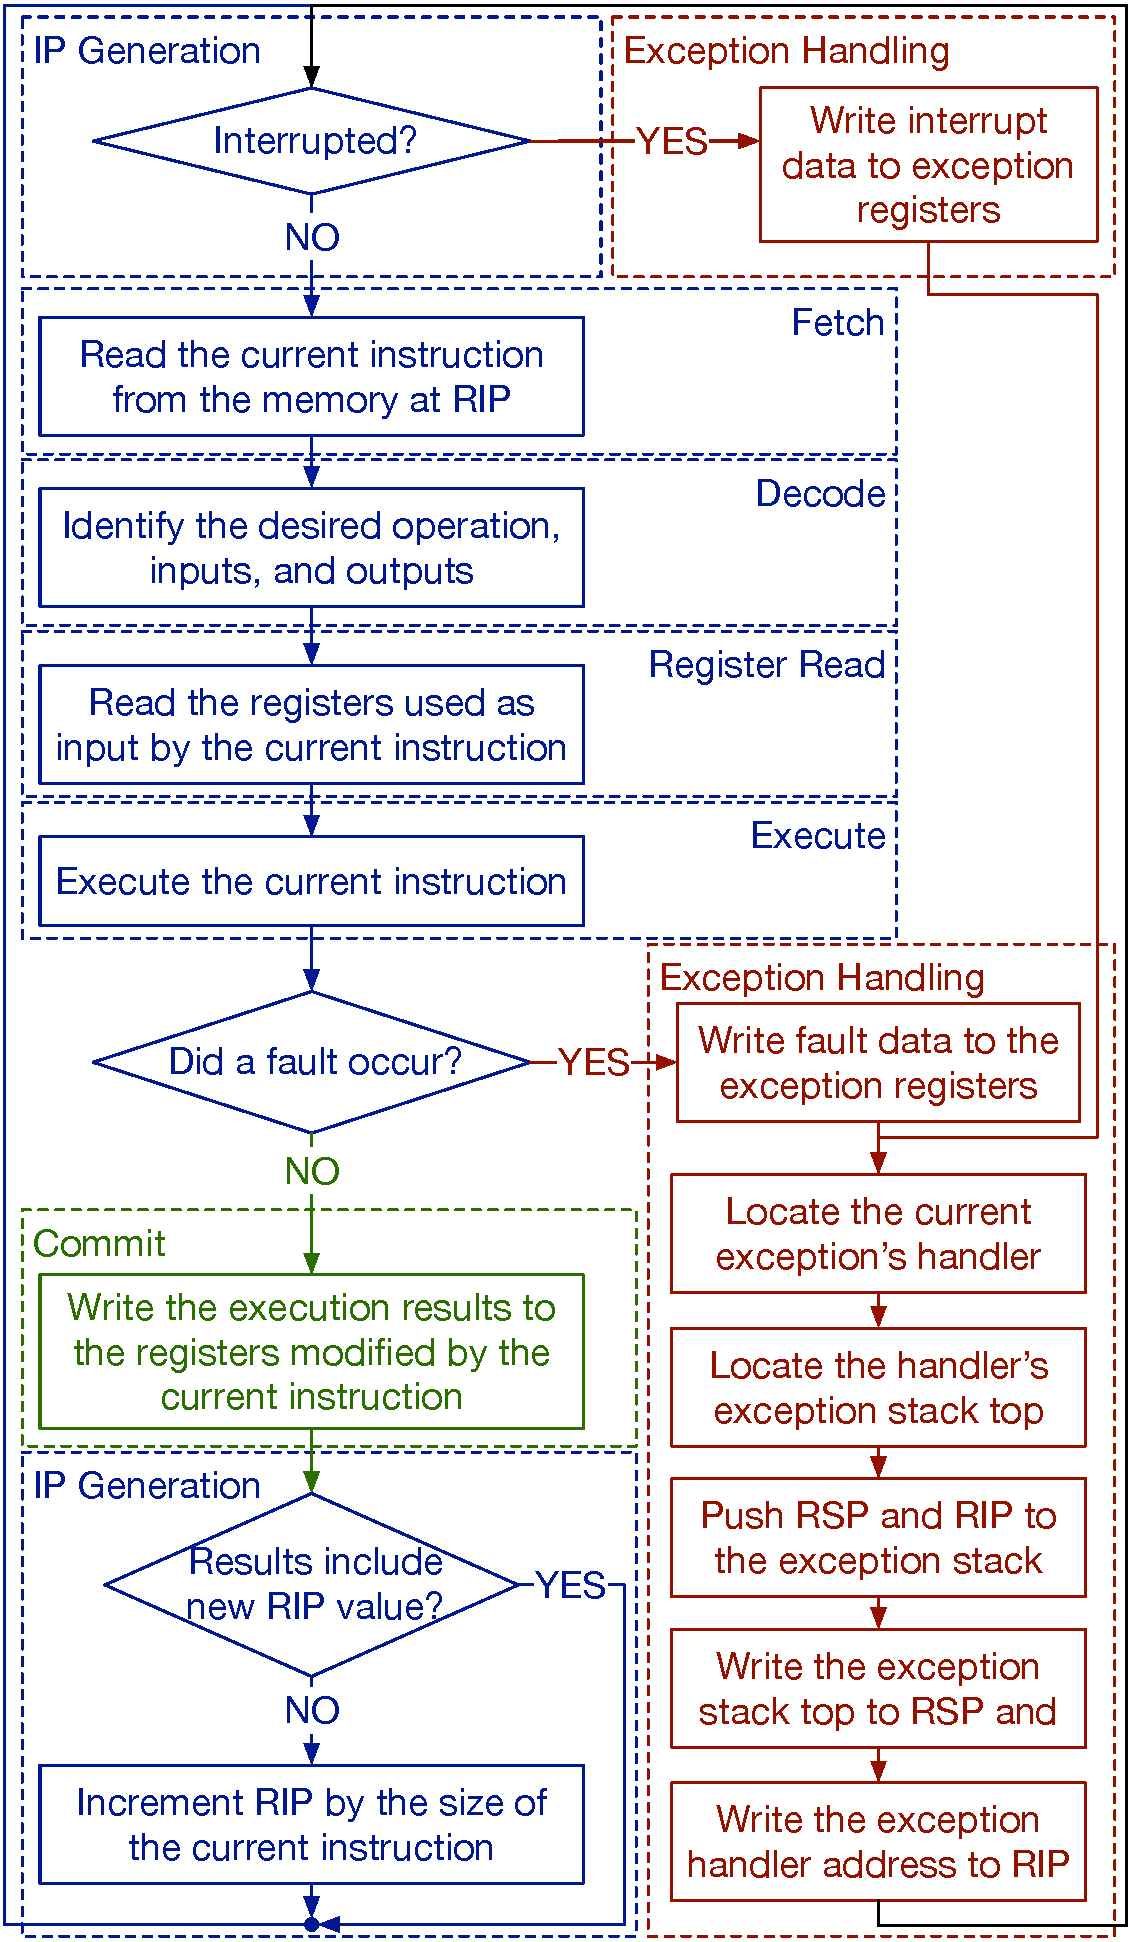
\includegraphics[width=85mm]{figures/processor_execution.pdf}
  \caption{
    A processor fetches instructions from the memory and executes them. The RIP
    register holds the address of the instruction to be executed.
  }
  \label{fig:processor_execution}
\end{figure}

The processor has an internal memory, referred to as the
\textit{register file}. The register file's memory cells, generally known as
\textit{registers}, make up the \textit{execution context} used to execute
instructions.

The registers mentioned in Figure~\ref{fig:processor_execution} are the
\textit{instruction pointer}~(RIP), which stores the memory  address of the
next instruction to be executed by the processor, and the
\textit{stack pointer}~(RSP), which stores the memory address of the topmost
element in the call stack used by the processor's procedural programming
support. The other execution context registers are described in
\S~\ref{sec:address_spaces} and \S~\ref{sec:registers}.

Under normal circumstances, the processor repeatedly reads the instruction at
the address in RIP, executes it, and updates RIP to point to the instruction
following the executed instruction. Unlike many RISC architectures, the Intel
architecture uses a variable-size instruction encoding, so the size of an
instruction is not known until the instruction has been fully read.

Some times, the processor encounters an exceptional conditions, called
\textit{faults}, while executing an instruction. For example, an integer
division instruction \texttt{DIV} where the divisor is zero does not have a
well-defined result, so its result is a Division Fault (\#DIV).

When executing an instruction results in a fault, the processor stops its
normal execution flow, and performs the fault handler process documented in
\S~\ref{sec:faults}. In a nutshell, the processor first looks up the address of
the code that will handle the fault, based on the fault's nature, and sets up
the execution environment in preparation to execute the fault handler.

The processors are connected to each other and to the memory via a
\textit{system bus}, which is a broadcast network that implements the
abstraction in Figure~\ref{fig:bus_abstraction}.

\begin{figure}[hbt]
  \centering
  \begin{tabularx}{\columnwidth}{| X |}
  \hline
  \textsc{send}(\textit{op}, \textit{addr}, \textit{data})
  $ \rightarrow \varnothing $ \\
  Place a message containing the operation code \textit{op}, the bus address
  \textit{addr}, and the value \textit{data} on the bus. \\
  \hline
  \textsc{read}() $ \rightarrow $ (\textit{op}, \textit{addr},
  \textit{value}) \\
  Return the message that was written on the bus at the beginning of this
  clock cycle. \\
  \hline
  \end{tabularx}
  \caption{The system bus abstraction}
  \label{fig:bus_abstraction}
\end{figure}

During each clock cycle, at most one of the devices connected to the system bus
can send a message, which is received by all the other devices connected to the
bus.

For example, when the processor wishes to read a memory location, it sends a
message with the operation code \textsc{read-request} and the bus address
corresponding to the desired memory location. The memory sees the message on
the bus and performs the \textsc{read} operation. At a later time, the memory
responds by sending a message with the operation code \textsc{read-response},
the same address as the request, and the data value set to the result of the
\textsc{read} operation.

The computer communicates with the outside world via I/O devices, such as
keyboards, displays, and network cards, which are connected to the system bus.
Devices mostly respond to requests issued by the processor. However, devices
also have the ability to issue \textit{interrupt requests} that notify the
processor of outside events, such as the user pressing a key on a keyboard.

Interrupt triggering is discussed in \S~\ref{sec:interrupts}. On modern
systems, devices send interrupt requests by issuing writes to special bus
addresses. The processor handles interrupt requests using
